% !TEX TS-program = xelatex
% !TEX encoding = UTF-8
\documentclass[a4paper, 12pt]{amsart}
\renewcommand\baselinestretch{1.2}
\usepackage{xeCJK, amsthm, tikz, algorithm, algorithmicx, algpseudocode,  amsaddr, hyperref}
%\usepackage[notref, notcite]{showkeys}
\setCJKmainfont[ItalicFont={KaiTi}, BoldFont={SimHei}]{SimSun}
\setCJKsansfont{SimHei}
\setCJKmonofont{FangSong}
\xeCJKsetup{AutoFakeSlant={true}, AutoFakeBold={true}}
\newcommand{\md}{\mathrm{d}}
\newcommand{\sgn}{\mathrm{sgn}}
\newcommand{\lr}[1]{\left(#1\right)}
\newcommand{\abs}[1]{\left\lvert#1\right\rvert}
\newcommand{\nm}[2]{\left\|\,#1\,\right\|_{#2}}
\numberwithin{equation}{section}
\newtheorem{theorem}{定理}[section]
\newtheorem{prop}[theorem]{命题}
\renewcommand\proofname{\bf 证明. }
%\renewcommand\emailaddrname{电子邮箱: }
\renewcommand\datename{时间: }
\renewcommand\tablename{表}
\renewcommand\figurename{图}
\floatname{algorithm}{算法}
\renewcommand{\algorithmicrequire}{\bf 输入: }
\renewcommand{\algorithmicensure}{\bf 输出: }

\begin{document}
\title[Burgers Equation]{Burgers 方程的守恒型格式求解}
\author[Y.L. Liao]{廖钰蕾}
\address{数学与系统科学研究院计算数学与科学工程计算研究所\\
电子邮箱 {\tt: \url{liaoyulei19@mails.ucas.ac.cn}}
}
%\email{liaoyulei19@mails.ucas.ac.cn}
\date{2019年11月30日}
\maketitle

\section{\bf 问题描述}\hspace*{\fill}\par
对下述Burgers 方程的初边值问题
\begin{equation}\label{eq:Burgers}\begin{cases}
u_t+(u^2/2)_x=0,\quad x\in[-1,1],\quad t>0,\\
u(x,0)=u_0(x)=\sin(\pi x+\pi),\\
\text{periodic }B.C.\text{ for }x,
\end{cases}\end{equation}
使用不同的守恒型格式求解. 包括Lax-Friedrichs, Roe(迎风), Engquist-Osher格式, Godunov格式, 和Lax-Wendroff格式.
\begin{itemize}
\item 计算各个格式在$t=0.15$时的误差和收敛阶.
\item 画出$t=0.5$时的精确解和数值解对比图.
\end{itemize}

\hspace*{\fill}\par\section{\bf 关键算法和格式}
\subsection{精确解求解方法}\hspace*{\fill}\par\hspace*{\fill}\par
利用特征线可以计算守恒律方程的精确解. Burgers 方程~\eqref{eq:Burgers}的特征线如图~\ref{fig:chr}所示.
\begin{figure}[htbp]\centering\begin{tikzpicture}
\draw[->](-2.5,0)--(2.5,0);
\node[below]at(2.5,0){$x$};
\draw[->](0,-0.5)--(0,1.5);
\node[left]at(0,1.5){$t$};
\node[below left]at(0,0){0};
\node[left]at(0,1){0.5};
\draw[->](-2,0)--(-2,1);
\node[below]at(-2,0){-1};
\draw[->](-1.5,0)--(-0.8,1);
\draw[->](-1,0)--(0,1);
\node[below]at(-1,0){-0.5};
\draw[->](-0.5,0)--(0,0.7);
\draw[->](0.5,0)--(0,0.7);
\draw[->](1,0)--(0,1);
\node[below]at(1,0){0.5};
\draw[->](1.5,0)--(0.8,1);
\draw[->](2,0)--(2,1);
\node[below]at(2,0){1};
\end{tikzpicture}\caption{Burger方程~\ref{eq:Burgers}的特征线}\label{fig:chr}\end{figure}

\begin{prop}
Burgers 方程~\eqref{eq:Burgers}仅在$x=0$处出现激波, 无稀疏波. 
\end{prop}

\begin{proof}
考虑过点$(x_0,0)$的特征线$x=x_0-\sin(\pi x_0)t$与$x=0$交于$t=x_0/\sin(\pi x_0)$处. 令
\[f(x_0):=\dfrac{x_0}{\sin(\pi x_0)},\quad x_0\in[-1,1],\]
求导得
\[f'(x_0)=\dfrac{\sin(\pi x_0)-\pi x_0\cos(\pi x_0)}{\sin^2(\pi x_0)}.\]
令
\[g(x_0):=\sin(\pi x_0)-\pi x_0\cos(\pi x_0),\]
求导得
\[g'(x_0)=\pi^2x_0\sin(\pi x_0)\ge 0,\quad x_0\in[-1,1].\]
由$g(0)=0$知, $f(x_0)$在$x_0\in(-1,0)$单调递减, 在$x_0\in(0,1)$单调递增. 故特征线仅在$x_0=0$处相交.
\end{proof}

若点$(x,t)$处精确解为$u$, 则过该点的特征线$x'=x+u(t'-t)$交$t_0=0$于点$x_0=x-ut$处, 且在$(x_0,0)$处的精确解$u_0(x-ut)=-\sin(\pi(x-ut))$. 故点$(x,t)$处精确解$u$满足方程
\[f(u):=u+\sin(\pi(x-ut))=0.\]

我们采用Newton 迭代法计算点$(x,t)$处精确解$u$, 迭代初值设为$-\sgn(x)$, 其中$\sgn(\cdot)$为符号函数. 具体过程见算法~\ref{alg:exact}.
\begin{algorithm}[htbp]\caption{计算精确解算法}\label{alg:exact}\begin{algorithmic}
\Require 空间坐标$x[1:n]$, 时间坐标$t$, 精度$tgv$.
\Ensure 精确解$u[1:n]$.
\Function{ExSolu}{$x, t, tgv$}
	\State 设置初值$u\gets-\sgn(x)$
	\State 待求$f(u)\gets u+\sin(\pi(x-ut))$的零点
	\While{$\nm{f(u)}{\infty}>tgv$}
		\State 进行一次Newton 迭代$u\gets u-f(u)/f'(u)$
		\State $f(u)\gets u+\sin(\pi(x-ut))$
	\EndWhile
	\State\Return $u$
\EndFunction
\end{algorithmic}\end{algorithm}

\hspace*{\fill}\par\subsection{数值解计算格式}\hspace*{\fill}\par\hspace*{\fill}\par
我们采用守恒型格式
	\[u_j^{n+1}=u_j^n-\dfrac{\Delta t}{\Delta x}\lr{\Hat{f}_{j+1/2}-\Hat{f}_{j-1/2}}\]
计算数值解. 对于不同的守恒型格式, 通量$\Hat{f}_{j+1/2}$不同. 

Burgers 方程~\eqref{eq:Burgers}不含$x=\pm1$的边值条件. 由于$t=0$的初值条件是周期的, 当网格划分均匀时, 每个时间层计算的数值解也是周期的, 即$u[n]=u[1],u[n+1]=u[2],\dots.$可由此计算边界的数值解, 具体算法如~\ref{alg:numer}, 其中$\Hat{f}_{j+1/2}$为上述通量.

\begin{algorithm}[htbp]\caption{计算数值解算法}\label{alg:numer}\begin{algorithmic}
\Require 初值$u_0[1:n]$, 空间坐标$x[1:n]$, 空间间隔$dx$, 时间间隔$dt$, 时间层$nt$, 通量函数$\Hat{f}_{j+1/2}(u)$.
\Ensure 数值解$u[1:n]$.
\Function{NuSolu}{$u_0,x,dx,dt,nt$}
	\State 由周期性扩展初值$u\gets[u_0,u_0[2]]$
	\For{$it=1:nt$}
		\State $hatf[j]\gets\Hat{f}_{j+1/2}(u),\quad j=1,\dots,n$
		\State $u[2:n]\gets u[2:n]-dt/dx*(hatf[2:n]-hatf[1:n-1])$
		\State $u[1]\gets u[n]$
		\State $u[n+1]\gets u[2]$
	\EndFor
	\State\Return $u$
\EndFunction
\end{algorithmic}\end{algorithm}

Burgers 方程~\eqref{eq:Burgers}中$f(u)=u^2/2$, 对应的不同格式通量如下:
\begin{itemize}
\item Lax-Friedrichs:
\[\Hat{f}_{j+1/2}=\dfrac12\lr{\dfrac12u_j^2+\dfrac12u_{j+1}^2-\dfrac{\Delta x}{\Delta t}\lr{u_{j+1}-u_j}}.\]
\item Roe:
\[\Hat{f}_{j+1/2}=\begin{cases}
u_j^2/2,\quad&u_j+u_{j+1}\ge0,\\
u_{j+1}^2/2,\quad&u_j+u_{j+1}<0.
\end{cases}\]
\item Engquist-Osher:
\[\Hat{f}_{j+1/2}=\dfrac12\lr{\max(u_j,0)}^2+\dfrac12\lr{\min(u_{j+1},0)}^2.\]
\item Godunov:
\[\Hat{f}_{j+1/2}=\begin{cases}
\min(u_j^2,u_{j+1}^2)/2,\quad&u_j<u_{j+1}\text{ 且 }u_{j}u_{j+1}>0,\\
\max(u_j^2,u_{j+1}^2)/2,\quad&u_j\ge u_{j+1},\\
0,\quad&\text{否则}.
\end{cases}\]
\item Lax-Wendroff:
\[\Hat{f}_{j+1/2}=\dfrac12\lr{\dfrac12(u_j^2+u_{j+1}^2)-\dfrac{\Delta t}{4\Delta x}\lr{u_j+u_{j+1}}\lr{u_{j+1}^2-u_j^2}}.\]
\end{itemize}

\hspace*{\fill}\par\section{\bf 数值实验}\hspace*{\fill}\par
我们的实验使用GNU Octave v5.1.0~\footnote{\url{https://www.gnu.org/software/octave/doc/v5.1.0/}}实现, 运行系统为Windows10-x64. 

守恒型格式的稳定性必要条件为$(\Delta t/\Delta x)\max_u\abs{f'(u)}\le 1$, 其中Burgers方程~\eqref{eq:Burgers}的$f(u)=u^2/2$. 由于$\max_u\abs{f'(u)}=1$, 实验中我们取$\Delta t/\Delta x=1$. 计算精确解$u$时, Newton 迭代法的终止条件为$\nm{f(u)}{\infty}\le\text{1e-10}$.

\hspace*{\fill}\par\subsection{第一个数值实验}\hspace*{\fill}\par\hspace*{\fill}\par
我们计算$t=0.15$时上述五种守恒型格式的误差和收敛阶, 实验结果见表~\ref{tab:task1}, 其中表头为网格细度$\Delta t=\Delta x$的值. 可以看出Lax-Friedrichs, Roe, Engquist-Osher, Godunov 的收敛阶为1, 其中Lax-Friedrichs 解的精度更低, 验证了其相比迎风格式有更大耗散性的特点. Lax-Wendroff的收敛阶为2, 解有更高的精度.

\begin{table}[htbp]\centering\caption{$t=0.15$时的误差和收敛阶, 表头为$\Delta t=\Delta x$的值}\label{tab:task1}
\begin{tabular}{ccccccc}
\hline\hline
1/40 & 1/80 & 1/160 & 1/320 & 1/640 & 1/1280\\
\hline\hline
\multicolumn{6}{l}{Lax-Friedrichs}\\
2.450e-2 & 1.249e-2 & 6.317e-3 & 3.177e-3 & 1.594e-3 & 7.982e-4\\
rate & 0.97 & 0.98 & 0.99 & 1.00 & 1.00\\ 
\hline
\multicolumn{6}{l}{Roe}\\
9.130e-3 & 5.002e-3 & 2.634e-3 & 1.354e-3 & 6.865e-4 & 3.457e-4\\
rate & 0.87 & 0.93 & 0.96 & 0.98 & 0.99\\
\hline
\multicolumn{6}{l}{Engquist-Osher}\\
9.130e-3 & 5.002e-3 & 2.634e-3 & 1.354e-3 & 6.865e-4 & 3.457e-4\\
rate & 0.87 & 0.93 & 0.96 & 0.98 & 0.99\\
\hline
\multicolumn{6}{l}{Godunov}\\
9.130e-3 & 5.002e-3 & 2.634e-3 & 1.354e-3 & 6.865e-4 & 3.457e-4\\
rate & 0.87 & 0.93 & 0.96 & 0.98 & 0.99\\
\hline
\multicolumn{6}{l}{Lax-Wendroff}\\
1.519e-3 & 3.904e-4 & 9.858e-5 & 2.477e-5 & 6.204e-6 & 1.553e-6\\
rate & 1.96 & 1.99 & 1.99 & 2.00 & 2.00\\
\hline\hline
\end{tabular}\end{table}

\hspace*{\fill}\par\subsection{第二个数值实验}\hspace*{\fill}\par\hspace*{\fill}\par
我们绘制了$t=0.5$时精确解和上述五种守恒型格式数值解对比图如下, 其中网格细度$\Delta t=\Delta x=1/256$. 可以看出Lax-Friedrichs, Roe, Engquist-Osher, Godunov 保持总变差不增, 符合单调格式的特点. Lax-Wendroff格式精度与收敛阶更高, 但在间断附近会产生震荡.
\begin{figure}[htbp]\centering
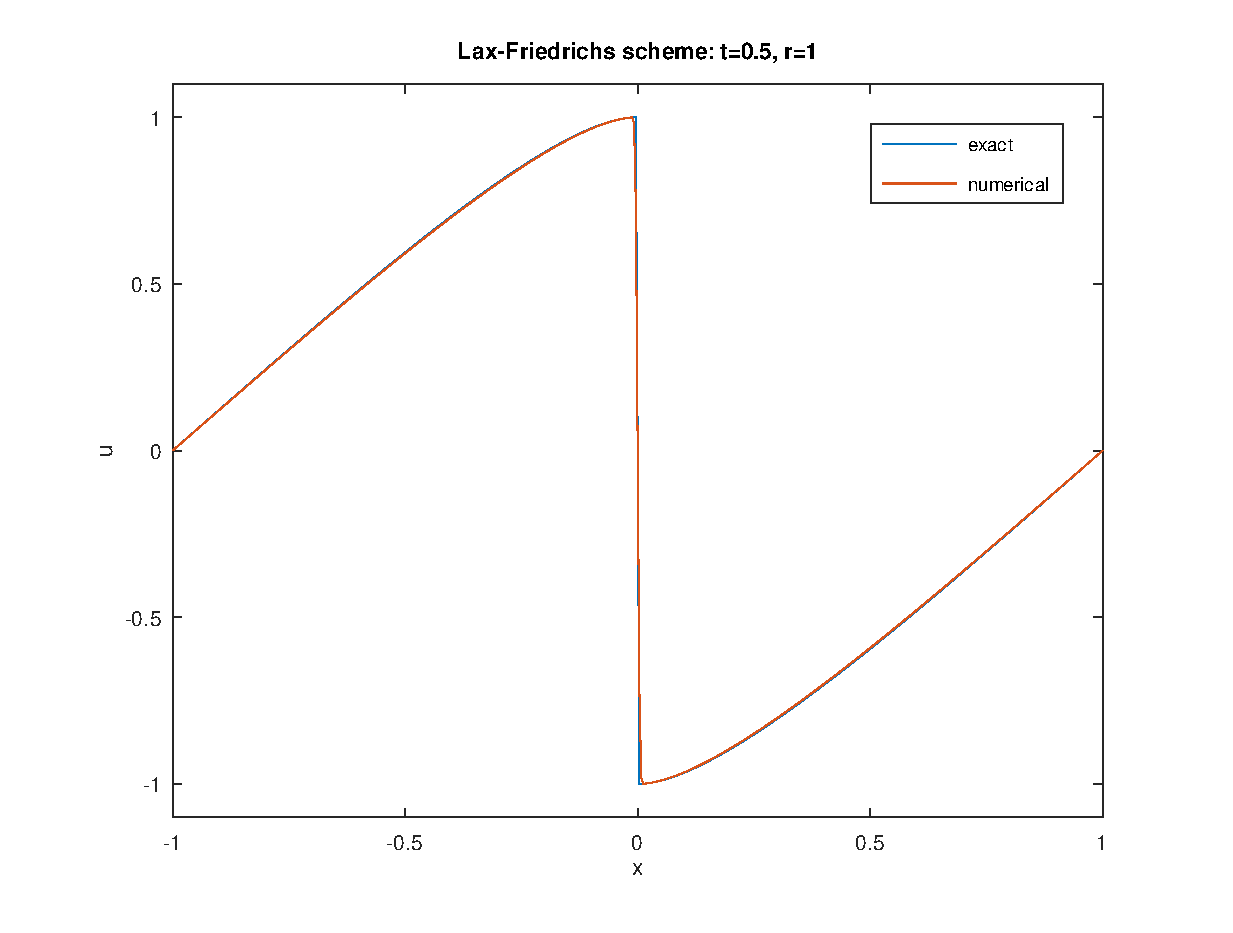
\includegraphics[width=\textwidth]{Lax-Friedrichs.eps}
\caption{$t=0.5$时Lax-Friedrichs 格式对比图}
\end{figure}

\begin{figure}[htbp]\centering
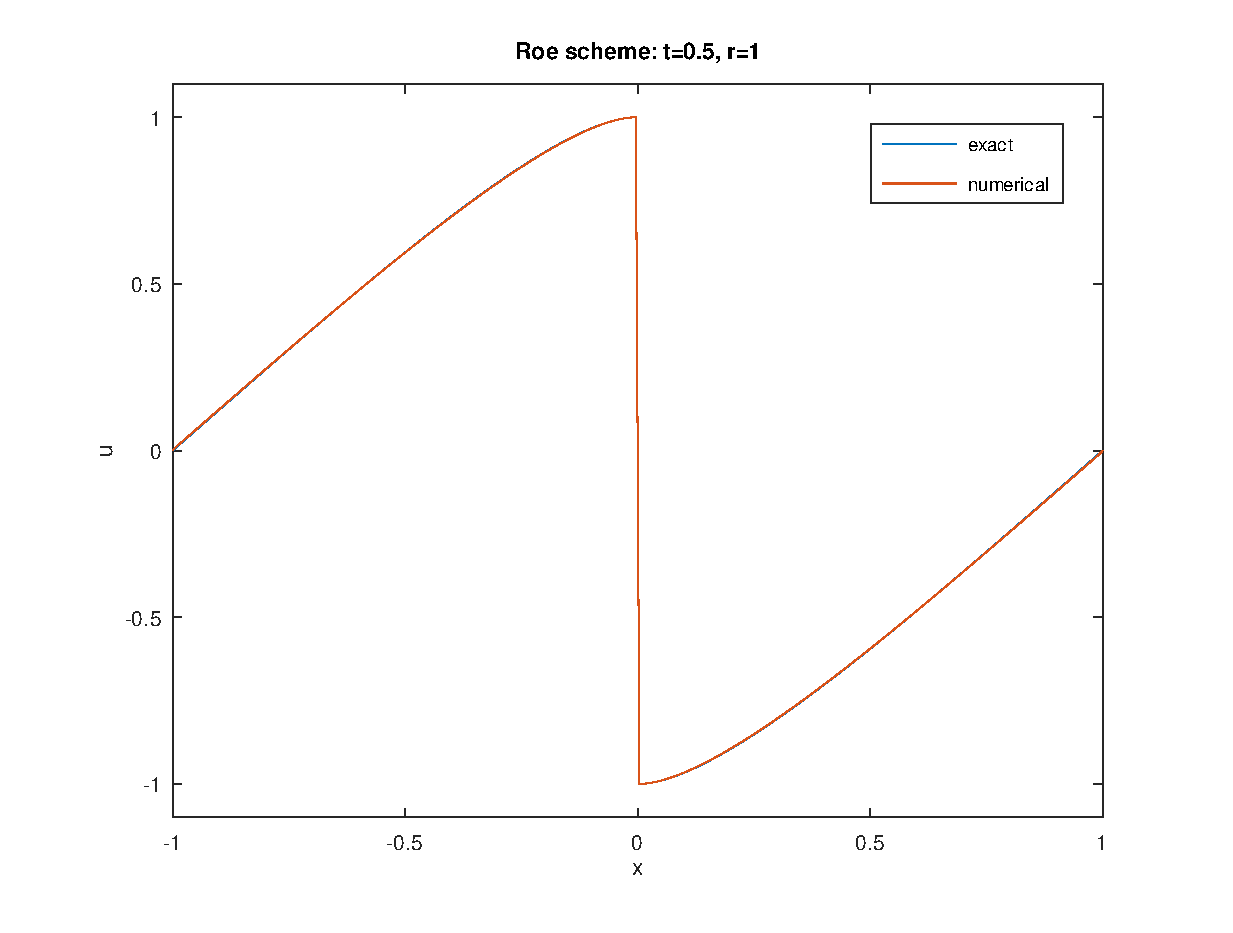
\includegraphics[width=\textwidth]{Roe.eps}
\caption{$t=0.5$时Roe 格式对比图}
\end{figure}

\begin{figure}[htbp]\centering
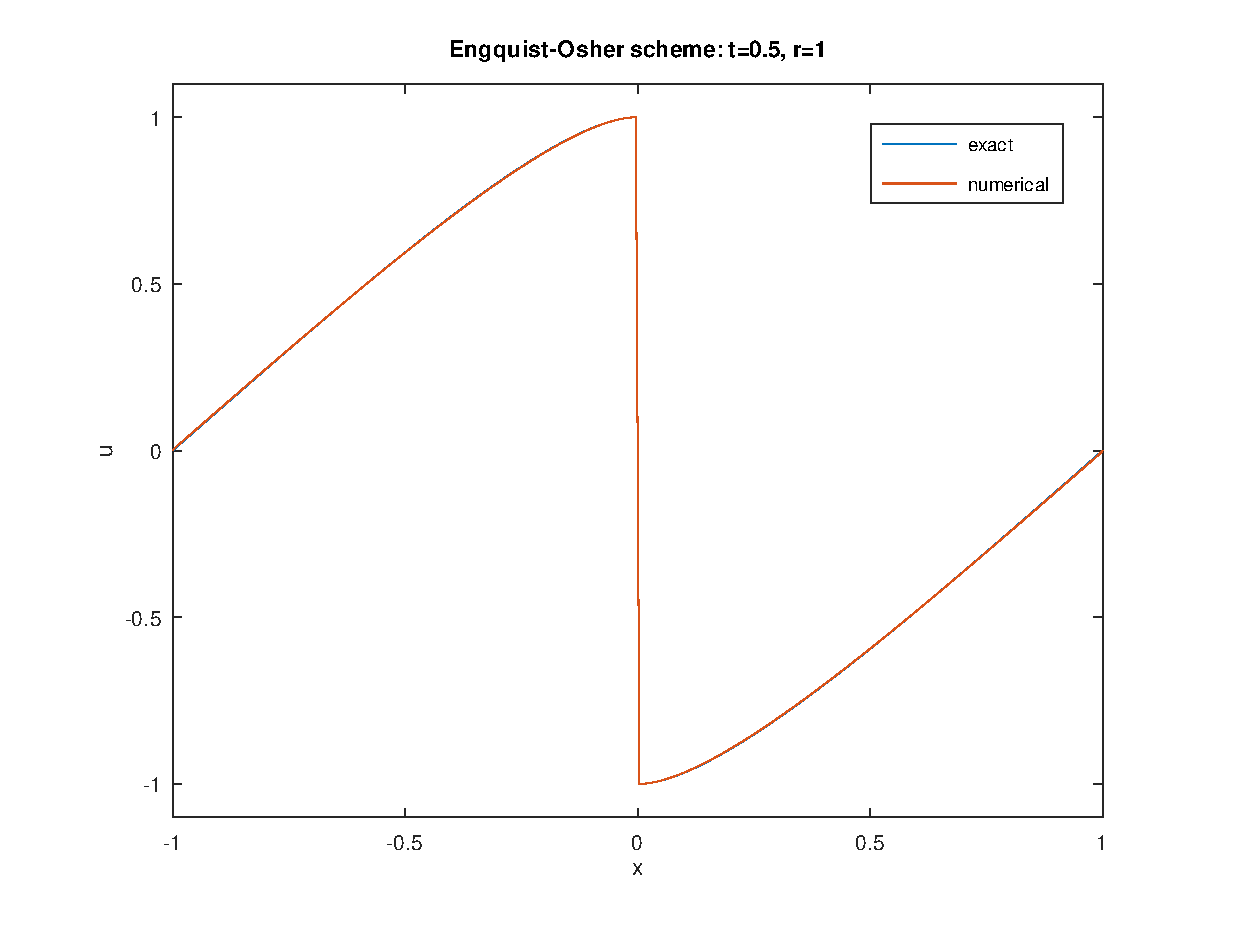
\includegraphics[width=\textwidth]{Engquist-Osher.eps}
\caption{$t=0.5$时Engquist-Osher 格式对比图}
\end{figure}

\begin{figure}[htbp]\centering
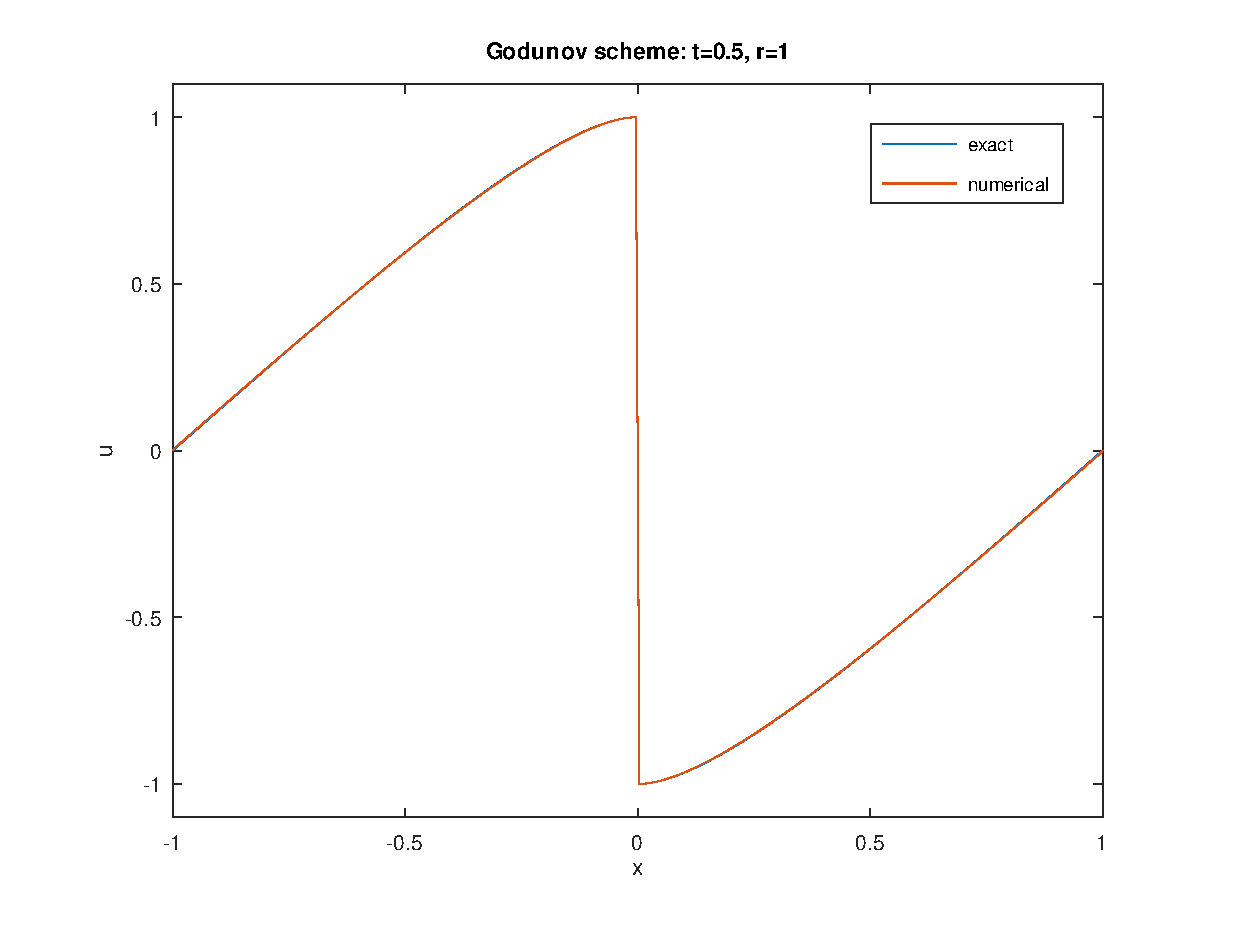
\includegraphics[width=\textwidth]{Godunov.eps}
\caption{$t=0.5$时Godunov 格式对比图}
\end{figure}

\begin{figure}[htbp]\centering
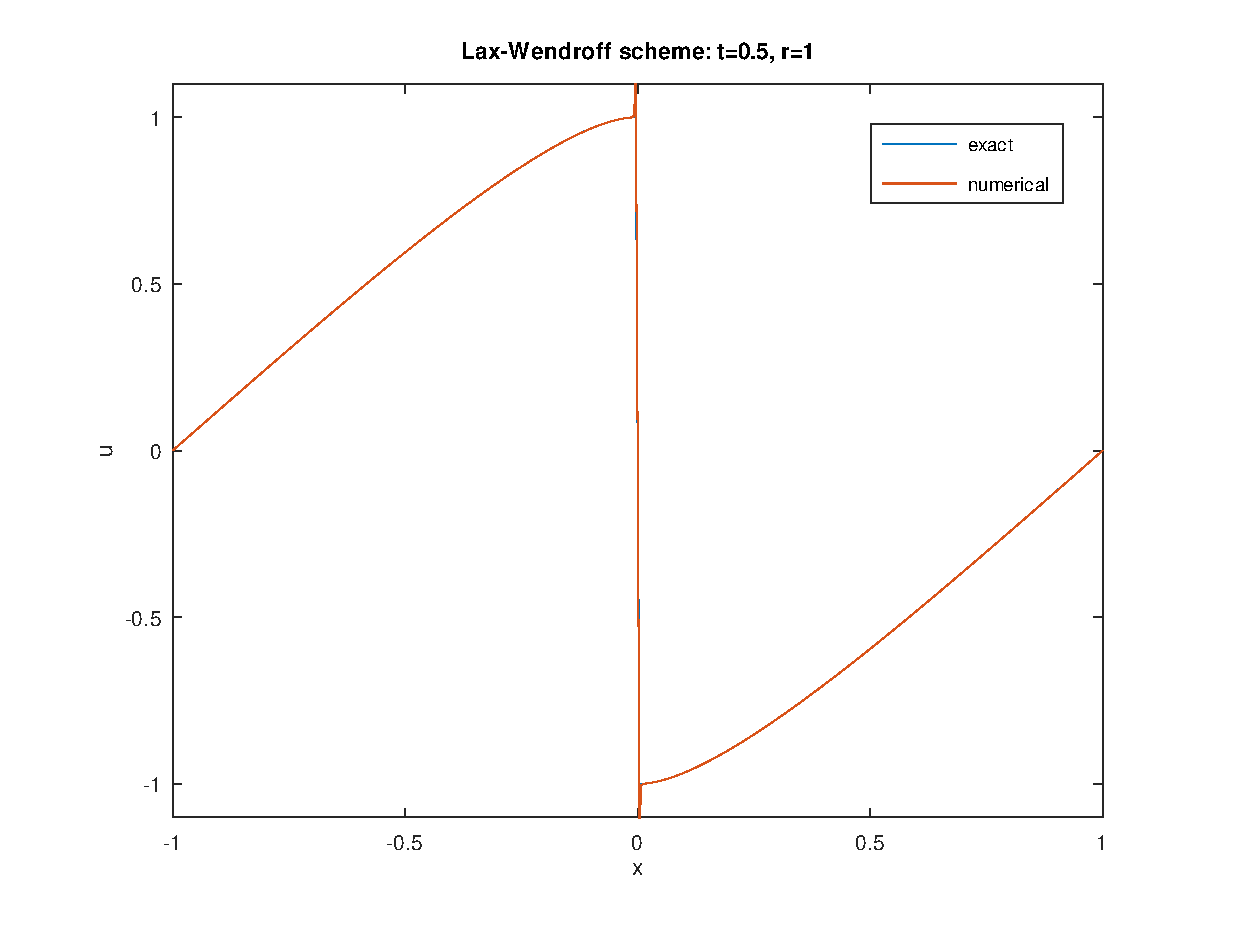
\includegraphics[width=\textwidth]{Lax-Wendroff.eps}
\caption{$t=0.5$时Lax-Wendroff 格式对比图}
\end{figure}

\end{document}